\chapter{Databases}

\exercise{3.3}
Discussed in person.

\exercise{3.9}
Check that $\Free(G)$ is a category for any graph $G$.

\solution
It is clear that concatenating any path with the trivial path yields the original, so unitality is satisfied.  Concatenation of paths is also associative (you can think of paths as lists of vertices/edges, which makes this clear).

\exercise{3.10}
Discussed in person

\exercise{3.12}
\begin{enumerate}
	\item What is the category $\textbf{1}$?
	\item What is the category $\textbf{0}$?
	\item What is the formula for the number of morphisms in $\textbf{n}$ for arbitrary $n\in\N$?
\end{enumerate}

\solution
\begin{enumerate}
	\item $\textbf{1}$ has a single object and only the identity morphism; it corresponds to the free category on the graph with one vertex.
	\item $\textbf{0}$ has no objects and no morphisms.
	\item The number of morphisms is $\sum_{i=1}^n i = \frac{n(n+1)}{2}$.  This is because there is one path of length $n-1$, two of length $n-2$, and so on until you get $n$ paths of length 1.
\end{enumerate}

\exercise{3.15}
In the loop graph, we identified paths with numbers $n\in\N$.  Given $m,n\in\N$, what number corresponds to the concatenation of their associated paths?

\solution
The concatenation corresponds to $m+n$.

\exercise{3.16}
\begin{enumerate}
	\item Write down the 10 paths in the free square category.
	\item Name two distinct parallel paths.
	\item Name two paths that are not parallel.
\end{enumerate}

\solution
\begin{enumerate}
	\item $\id_A, \id_B, \id_C, \id_D, f, g, h, i, f\fcmp h, g\fcmp i$
	\item $f\fcmp h$ and $g\fcmp i$
	\item $f$ and $g$
\end{enumerate}

\exercise{3.17}
See text.

\solution
This has the same morphisms as the commutative square, so $\{A, B, C, D, f ,g, h, i, f\fcmp h\}$.

\exercise{3.19}
See text.

\solution
$\{z, s, s\fcmp s, s\fcmp s\fcmp s\}$

\exercise{3.21}
See text.

\solution
$G_1$: $f=g$

$G_2$: $f=\id$

$G_3$: $f\fcmp h=g\fcmp i$

$G_4$: none

\exercise{3.22}
What is the preorder reflection of the category $\N$?

\solution
The preorder reflection of $\N$ is just the category with one object and its identity morphism.

\exercise{3.25}
Discussed in person.

\exercise{3.30}
\begin{enumerate}
	\item What is the inverse $f^{-1}:\underline{3}\to A$ of the function $f$ given in Example 3.29?
	\item How many distinct isomorphism are there $A\to\underline{3}$?
\end{enumerate}

\solution
\begin{enumerate}
	\item $f^{-1}(1) = b, f^{-1}(2)=a, f^{-1}(3)=c$
	\item This is just the number of permutations of a set of three elements, namely $3!=6$.
\end{enumerate}

\exercise{3.31}
Show that in any category $\mcC$, for any given object $c\in\mcC$, the identity $\id_c$ is an isomorphism.

\solution
By definition $\id_c\fcmp\id_c=\id_c$, so it's clearly an isomorphism.

\exercise{3.32}
A monoid in which every morphism is an isomorphism is a group.
\begin{enumerate}
	\item Is the monoid in Example 3.13 a group?
	\item Is the monoid in Example 3.18 a group?
\end{enumerate}

\solution
\begin{enumerate}
	\item $\N$ is not a group, as for example $s$ is not an isomorphism.  This is because $s$ composed with any element of the set of paths $\{z,s, s\fcmp s,\dots\}$ yields the set $\{s, s\fcmp s, s\fcmp s\fcmp s,\dots\}$, of which $z$ is clearly not a member.
	\item $\mcC$ is a group.  There are only two morphisms: the identity $z$ which is an isomorphism, and $s$ where $s\fcmp s=z$ making it an isomorphism as well.
\end{enumerate}

\exercise{3.33}
Let $G$ be a graph and $\Free(G)$ the corresponding free category.  Is it true that the only isomorphism in $\Free(G)$ are the identity morphisms?

\solution
This is true, since there are no equations, so for any $f:A\to B$ with an accompanying $g:B\to A$, we don't necessarily have $f\fcmp g=\id_A$ or $g\fcmp f=\id_B$.

\exercise{3.37}
Find all the functors from $\textbf{2}\to\textbf{3}$.

\solution
This is almost the number of functions that we found in Exercise 3.25 but without any that flip elements, which leaves 6.

\exercise{3.39}
Say where each of the 10 morphisms in $\mcF$ is is sent under the functor $F$ from Example 3.38.

\solution
$F(\id_{X'})=\id_{X}$ for any $X\in\{A,B,C,D\}$

$F(y')=y$ for any $y\in\{f,g,h,i\}$

$F(f'\fcmp h')=F(g'\fcmp i')=f\fcmp h$

\exercise{3.40}
See text.

\solution
One functor takes the arrow in $\mcC$ to the top arrow in $\mcD$, the other takes it to the bottom arrow.

\exercise{3.43}
Show that there is a category $\Cat$, where the objects are categories and morphisms are functors.

\solution
First we define $\id_\mcC:\mcC\to\mcC$ as follows: for any $c\in\Ob(\mcC)$, $\id_\mcC(c)=c$ and for any $f\in\mcC(c,d)$, $\id_\mcC(f)=f\in\mcC(\id_\mcC(c),\id_\mcC(d))=\mcC(c,d)$.  This is a functor, because $\id_\mcC(\id_c) = \id_c=\id_{\id_\mcC(c)}$, and for any $f\in\mcC(c_1,c_2)$ and $g\in\mcC(c_2,c_3)$. we have $\id_\mcC(f\fcmp g)=f\fcmp g = \id_\mcC(f)\fcmp\id_\mcC(g)$.

Next we define composition of functors $F:\mcC\to\mcD$ and $G:\mcD\to\mcE$ as follows: for any $c\in\Ob(\mcC)$, $(F\fcmp G)(c) = G(F(c))$ and for any $f\in\mcC(c,d)$, $(F\fcmp G)(f) = G(F(f))$.  Then $F\fcmp G:\mcC\to\mcE$ is a functor due to the functoriality of $F$ and $G$.  In particular, we have
$$(F\fcmp G)(\id_c)=G(F(\id_c))=G(\id_{F(c)})=\id_{G(F(c))}=\id_{(F\fcmp G)(c)},$$
as well as
$$(F\fcmp G)(f\fcmp g)=G(F(f\fcmp g)) = G(F(f)\fcmp F(g)) = G(F(f))\fcmp G(F(g)) = (F\fcmp G)(f)\fcmp (F\fcmp G)(g).$$

Note that this composition is associative simply because function composition is associative.  Unitality holds because $\id_\mcC$ is the identity function on objects and morphisms, so $(\id_\mcC\fcmp F)(c)=F(c)$ and $(\id_\mcC\fcmp F)(f)=F(f)$ and similarly for $F\fcmp\id_\mcD$.  Therefore $\Cat$ is indeed a valid category.

\exercise{3.45}
For any functor $F:\textbf{1}\to\Set$ one can extract a set $F(1)$.  Show that for any set $S$, there is a functor $F_S:\textbf{1}\to\Set$ such that $F_S(1)=S$.

\solution
$F_S$ clearly preserves identities, and as $\textbf{1}$ only has the identity morphism is preserves composition as well.  Hence $F_S$ is a valid functor.

\exercise{3.48}
Discussed in person.

\exercise{3.55}
Show exactly how $\mcD^\mcC$ is a category.

\solution
Let $\alpha: F\to G$ and $\beta: G\to H$ be natural transformations.  We define the $c$-component of the composition to be $(\alpha\fcmp\beta)_c:F(c)\to H(c)$ by $(\alpha\fcmp\beta)_c = \alpha_c\fcmp\beta_c$.  This is a valid natural transformation as for any morphism $f:c\to d$ in $\mcC$, we have
\begin{align*}
	F(f)\fcmp (\alpha\fcmp\beta)_d &= F(f)\fcmp(\alpha_d\fcmp\beta_d)\\
	&= (\alpha_c\fcmp G(f))\fcmp \beta_d,
	\intertext{by associativity and the fact that $\alpha$ is a natural transformation, and similarly}
	&=\alpha_c\fcmp(\beta_c\fcmp H(f))\\
	&=(\alpha\fcmp\beta)_c\fcmp H(f).
\end{align*}
This composition rule for natural transformations is associative just because the underlying morphism composition is associative.

We define the identity natural transformation on a functor $F$ to be $\iota_F:F\to F$ where $(\iota_F)_c:F(c)\to F(c)$ is just $\id_c$.  This is clearly natural by the definition of the identity morphism.  Then for any natural transformation $\alpha:F\to G$, we have for every $c$
$$(\iota_F\fcmp \alpha)_c = (\iota_F)_c\fcmp \alpha_c = \id_c\fcmp\ \alpha_c = \alpha_c$$
and similarly for $(\alpha\fcmp\iota_G)_c$.  This means $\iota_F\fcmp\alpha=\alpha$ and $\alpha\fcmp\iota_G=\alpha$.  Hence $\mcD^\mcC$ is a category where the objects are functors, the morphisms are natural transformations, and composition and identity are as defined above.

\exercise{3.58}
Let $\mcC$ be an arbitrary category and $\mcP$ a preorder.  Consider the following statements:
\begin{enumerate}
	\item For any two functors $F,G:\mcC\to\mcP$, there is at most one natural transformation $F\to G$.
	\item For any two functors $F,G:\mcP\to\mcC$, there is at most one natural transformation $F\to G$.
\end{enumerate}
For each, if it is true, say why; if it is false, give a counterexample.

\solution
\begin{enumerate}
	\item This is true, since a preorder has only one morphism between any two objects, so there is only one choice for each component $\alpha_c:F(c)\to G(c)$.
	\item This is not true, for example if $\mcC$ is a category with two objects $c$ and $d$ and two parallel morphisms $f,g:c\to d$, then any functors from $\mcP$ have a choice of which morphism to map to.
\end{enumerate}

\exercise{3.62}
See text.

\solution
\begin{tabular}{c|cc}
\text { Arrow } & \text { source } & \text { target } \\
\hline Mngr & Employee & Employee \\
WorksIn & Employee & Department \\
Secr & Department & Employee \\
FName & Employee & string \\
DName & Department & string
\end{tabular}
\hspace{2cm}
\begin{tabular}{c|}
\text { Vertex } \\
\hline Employee \\
Department \\
string
\end{tabular}

\exercise{3.64}
See text.

\solution
If $\alpha_{\textrm{Arrow}}(a)=d$, then we must have $\alpha_{\textrm{Arrow}}(b)=e$, $\alpha_{\textrm{Vertex}}(1)=4$, and $\alpha_{\textrm{Vertex}}(2)=\alpha_{\textrm{Vertex}}(3)=5$.

\exercise{3.67}
Discussed in person.

\exercise{3.73}
\begin{enumerate}
	\item Given a morphism $f:X\to Y$ (in $\Set$), what morphism should $-\times B:X\times B\to Y\times B$ return?
	\item Given a morphism $f:X\to Y$, what morphism should $(-)^B:X^B\to Y^B$ return?
	\item Consider the function $+:\N\times\N\to\N$ which sends $(a,b)\mapsto a+b$.  Currying $+$, we get a certain function $p:\N\to\N^\N$.  What is $p(3)$?
\end{enumerate}

\solution
\begin{enumerate}
	\item $-\times B$ should return the morphism $(f,\id_B)$.
	\item $(-)^B$ should return the morphism (set function) that maps $g\in X^B$ to $g\fcmp f$.
	\item $p(3)$ is function that sends $n\in\N$ to $n+3$.
\end{enumerate}

\exercise{3.76}
Describe the functor $!:\mcC\to\textbf{1}$: where does it send each object and morphism?

\solution
$!$ sends every object to the unique object in $\textbf{1}$ and every morphism to the identity on that object.

\exercise{3.78}
See text.

\solution
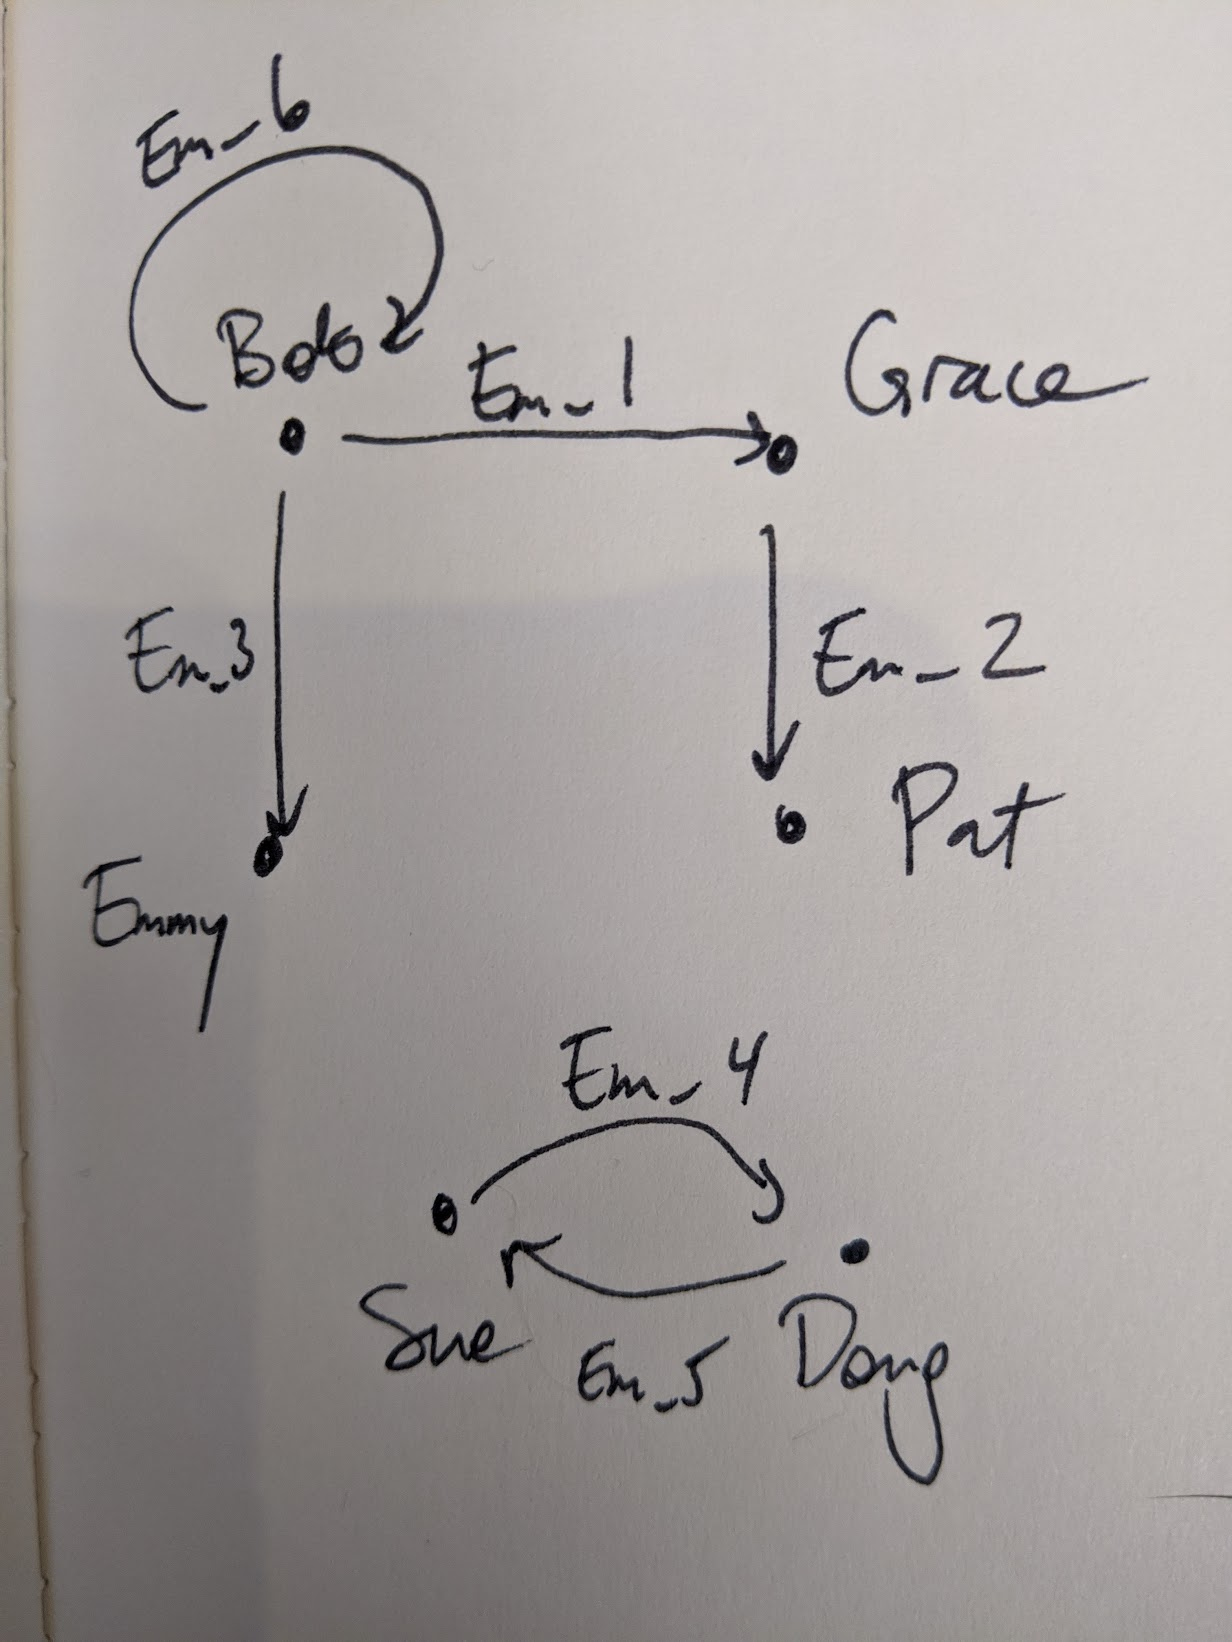
\includegraphics[width=0.5\textwidth]{images/3-78.jpg}

\exercise{3.81}
Let $(P,\leq)$ be a preorder, $z\in P$ an element and $\mcP$ the corresponding category.  Show that $z$ is a terminal object in $\mcP$ iff it is a top element in $P$: that is, for all $c\in P$ we have $c\leq z$.

\solution
By definition, we know $z$ is a terminal object if for every $c\in P$ we have a unique morphism $c\to z$.  But as there is only at most one morphism between any two objects in a preorder, namely $\leq$, this implies that $c\leq z$ for all $c\in P$.

\exercise{3.82}
Name a terminal object in $\Cat$.

\solution
Any category with a single object and a single morphism (the identity on that object) is a terminal object in $\Cat$.  This is due to Exercise 3.76.

\exercise{3.83}
Find a category that doesn't have a terminal object.

\solution
The schema $\textbf{Gr}$ from before is a category without a terminal object.  Arrow cannot be terminal as there is nor morphism from Vertex to Arrow, and Vertex cannot be terminal as there are two distinct morphisms from Arrow to Vertex.

\exercise{3.88}
Let $(P,\leq)$ be a preorder, let $x,y\in P$ be elements, and let $\mcP$ be the corresponding category.  Show that the product $x\times y$ in $\mcP$ agrees with their meet $x\land y$ in $P$.

\solution
Note that for a preorder, we need only show that a morphism exists to have a unique morphism between objects as there can only be at most one.

By definition, $x\land y \leq x,y$, which gives us the projection morphisms $p_x$ and $p_y$ in the definition of the product.  Also for any $c\in P$ where $c\leq x$ and $c\leq y$, we know that $c\leq x\land y$, giving us the unique morphism $\langle f,g\rangle$.  Hence the meet exactly corresponds to the product.

\exercise{3.90}
\begin{enumerate}
	\item What are the identity morphisms in a product category $\mcC\times\mcD$?
	\item Why is composition in a product category associative?
	\item What is the product category $\textbf{1}\times\textbf{2}$?
	\item What is the product category $\mcP\times\mcQ$ when $P$ and $Q$ are preorders and $\mcP$ and $\mcQ$ the corresponding categories?
\end{enumerate}

\solution
\begin{enumerate}
	\item The identity morphisms are just pairs of identities $(\id_c,\id_d)$ for $c\in\Ob(\mcC)$ and $d\in\Ob(\mcD)$.
	\item Composition is associative simply because the underlying composition of morphisms in $\mcC$ and $\mcD$ is associative.
	\item 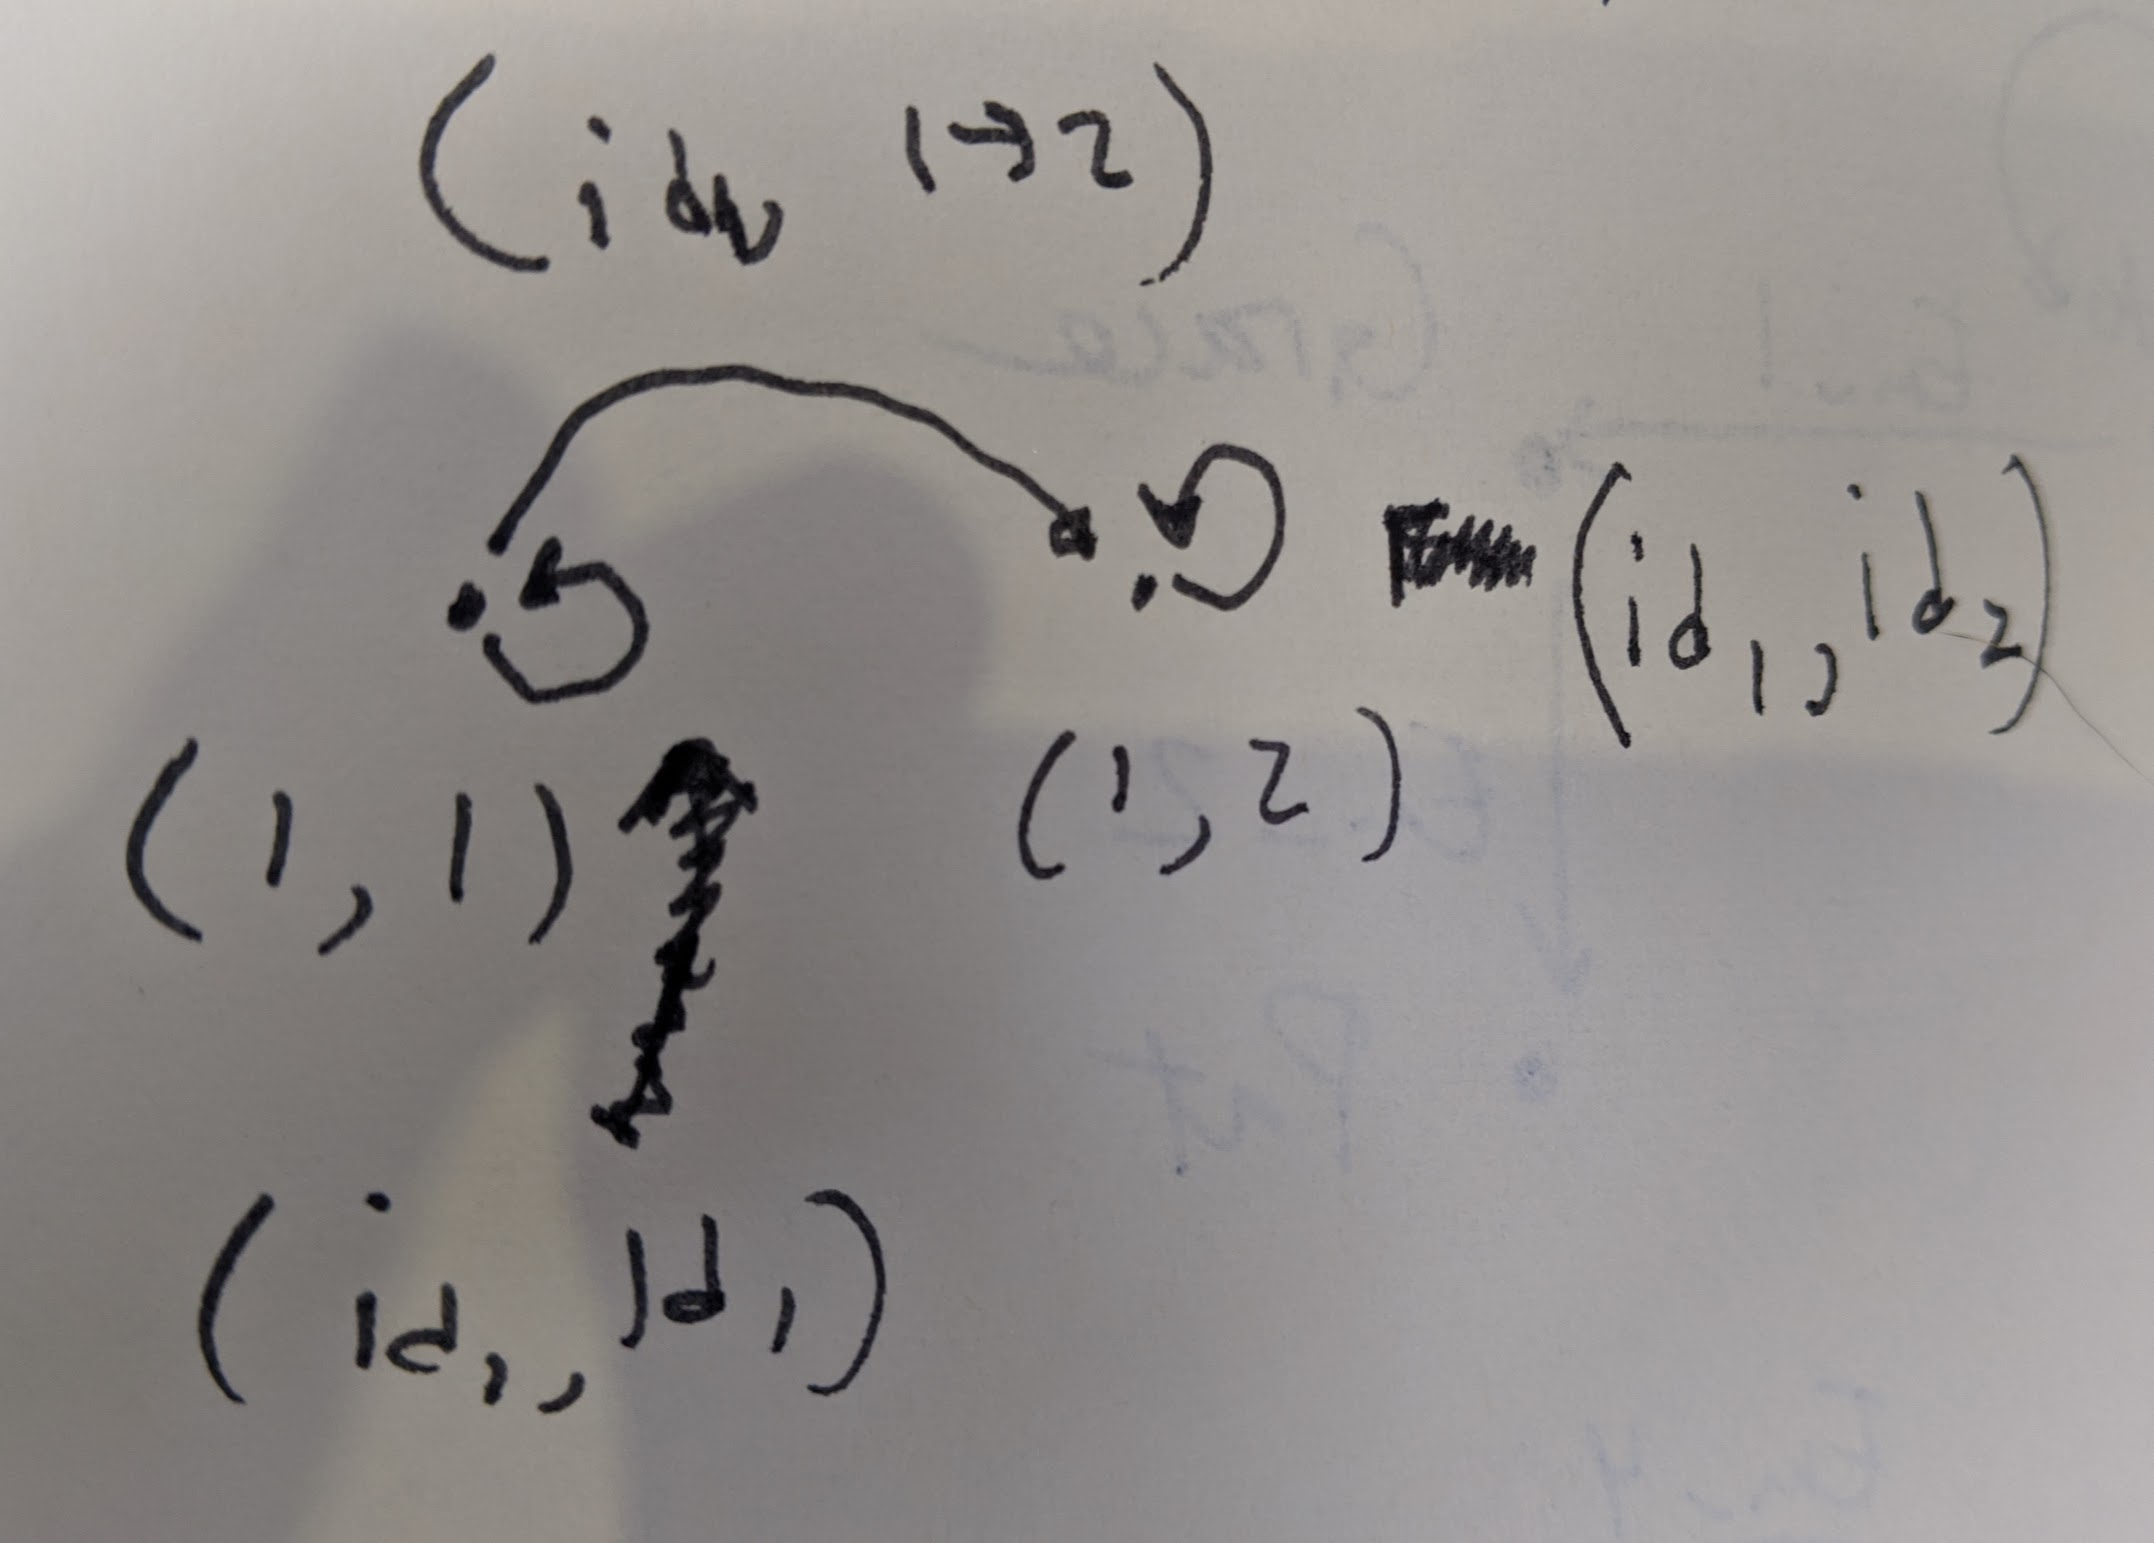
\includegraphics[width=0.5\textwidth]{images/3-90.jpg}
	\item $\mcP\times\mcQ$ has underlying set $P\times Q$ and a morphism $(p_1,q_1)\to(p_2,q_2)$ whenever $p_1\leq p_2$ and $q_1\leq q_2$.
\end{enumerate}

\exercise{3.91}
Check that a product $X\times Y$ is exactly the same as a terminal object in $\textbf{Cone}(X,Y)$.

\solution
$X\times Y$ is terminal if for every object in $\textbf{Cone}(X,Y)$, consisting of $C\in\Ob(\mcC)$ with  maps $f$ and $g$ to $X$ and $Y$ respectively, there is a unique cone morphism from $C\to X\times Y$.  But we have such a morphism from the definition of the product, namely $\langle f,g\rangle$, so $X\times Y$ is terminal.

\exercise{3.97}
Show that the limit formula in Theorem 3.95 works for products.

\solution
The product is the limit when the indexing category is just two objects and no non-identity morphisms (i.e. no arrows).  So the definition given in Theorem 3.95 gives the entire cartesian product of two sets.

\exercise{3.98}
If $D:\textbf{1}\to\Set$ is a functor, what is the limit of $D$?

\solution
Theorem 3.95 says that a limit of $D$ is just the set $D(\dot)$ where $\dot$ is the sole object in $\textbf{1}$.  We will show that any set $Z$ with a bijective function to $D(\dot)$ called $z_{\dot}$ is a terminal object in the cone category and hence a limit of $D$, which is compatible with the answer given by Theorem 3.95.

We show first that for any limit $(Z,z_{\dot})$, $|Z|\geq |D(\dot)|$.  To see this consider the cone $(D(\dot),id)$, as $(Z,z_{\dot})$ is a terminal object, there is a unique morphism $a:D(\dot)\to Z$, such that $id = a\fcmp z_{\dot}$.   As function application can only decrease the cardinality of a set we have $|\id(D(\dot)|= |(a\fcmp z_{\dot})(D(\dot)| \leq |Z|$. 

Secondly we show that for any limit $(Z,z_{\dot})$, $|Z|\leq |D(\dot)|$.  To see this suppose $(Q,q_{\dot})$ is an object in the cone category such that $|Q|> |D(\dot)|$.  As a result we must have that $q_{\dot}$ maps two elements to the same value in $D(\dot)$.  We can see two morphisms from $(Q,q_{\dot})$ to itself, the identity and the morphism which flips these two elements. 

Finally we show that for any $(Z,z_{\dot})$ which satisfies the properties above and any other object in the cone category $(C,c_{\dot})$, there exists a unique morphism from $(C,c_{\dot})$ to $(Z,z_{\dot})$.  Consider any morphism $a$, from $(C,c_{\dot})$ to $(Z,z_{\dot})$, we know by definition that $a\fcmp z_{\dot} = c_{\dot}$.  Thus as $z_{\dot}$ is invertible, we can also conclude $a = c_{\dot} \fcmp z_{\dot}^{-1}$, and it is uniquely defined by $(C,c_{\dot})$ and $(Z,z_{\dot})$.  We also note that for any $(C,c_{\dot})$ and $(Z,z_{\dot})$ this morphism exists, completing the proof.

\exercise{3.101}
Let $F:\mcC\to\mcD$ be a functor.  Define its opposite $F^{\opp}: \mcC^\opp\to\mcD^\opp$, i.e. how should it act on objects and morphisms?

\solution
$F^\opp$ should take an object $c$ in $\mcC^\opp$ (and hence also in $\mcC$) to $F(c)\in\Ob(\mcD^\opp)=\Ob(\mcD)$.

Next, for a morphism $f^\opp$ in $\mcC^\opp$, $F^\opp$ should take $f^\opp$ to $F(f)^\opp$ which we know must be a morphism in $\mcD^\opp$.

